\documentclass[
  letterpaper,
  twocolumn,
  9pt,
  journal,
  final]{IEEEtran}

\usepackage[spanish,es-tabla]{babel}
\usepackage[utf8]{inputenc}
\usepackage{amsfonts}
\usepackage{amsmath}
\usepackage{amssymb}
\usepackage{amsxtra}
\usepackage{mathrsfs}
\usepackage{array}
\usepackage{cite}
\usepackage{varioref}
\usepackage{float}
\usepackage{color}
\usepackage{colortbl}
\usepackage{enumerate}
\usepackage{rotating}
\usepackage{caption}
\usepackage{subcaption}
\usepackage{hyperref}
\usepackage{listings}
\usepackage{lipsum}
%\usepackage{flushend}
\usepackage{graphicx}
\usepackage{subcaption}

\title{Tarea 2 - Procesamiento Digital de Imágenes}
% \author{\textbf{Autor:} Pablo Yáñez Santibáñez - pablo.yanez@uai.com}
\author{
  \IEEEauthorblockN{Pablo Yáñez S.} - pablo.yanez@uai.cl
}

% Levels to show in table of contents:
% \setcounter{tocdepth}{-1} % only parts
% \setcounter{tocdepth}{0}  % only parts and chapters
\setcounter{tocdepth}{1}  % part,chapters,sections
% \setcounter{tocdepth}{2}  % part,chapters,sections, subsections
% \setcounter{tocdepth}{3}  % part,chapters,sections, subsections,subsubsections
% \setcounter{tocdepth}{4}  % part,chapters,sections, subsections,subsubsections and paragraphs
% \setcounter{tocdepth}{5}  % part,chapters,sections, subsections, subsubsections, paragraphs and subparagraphs.


\begin{document}
\bstctlcite{IEEEexample:BSTcontrol}

\maketitle

% \begin{abstract}
% We propose \lipsum[1]
% \end{abstract}

\tableofcontents

% \listoffigures

% \listoftables

%%%%%%%%%%%%%%%%%%%%%%%%%%%%%%%%%%%%%%%%%%%%%%%%%%%%%%%%%%%%%%%%%%%%%%%%%%%%%%%%
\vspace{-0.1cm}
\section{Marco Teórico}

Las imágenes digitales están compuestas por miles de unidades conocidas como pixeles.  Los dispositivos digitales generalmente usan el modelo RGB (Red-Green-Blue), el cual es un modelo de aditivo de colores que permite crear colores compuestos en base a la suma de sus colores primarios. La información contenida en uno de estos espacios de colores es lo que se conoce como canal.

\begin{figure}[!tbh]
  \begin{center}
    \resizebox{\columnwidth}{!}{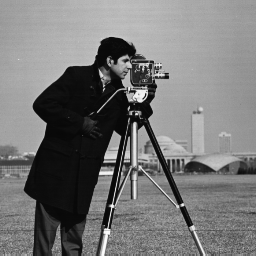
\includegraphics[trim={1cm 5cm 2cm 1.2cm},clip]{other/cameraman.png}}
  \end{center}
  \caption{Imagen en escala de grises \cite{carrasco1}.} \label{fig:cameraman}
\end{figure}


En el caso de las imágenes en escala de grises estas poseen solo un canal, lo que quiere decir que en vez de poseer tres valores distintos por cada pixel, solo posee un valor, el cual representa la cantidad de luz capturado en ese punto. El contraste varia desde el negro en las intensidades más bajas hasta el blanco en las intensidades más altas.

\subsection{Ecualización del histograma}

La ecualización de una imagen permite modificar una imagen cambiando la distribución de su histograma, tratando de distribuir las intensidades de forma uniforme. El resultado de este proceso es modificar el contraste de una imagen.

\begin{figure}[!tbh]
  \begin{center}
    \resizebox{0.9\columnwidth}{!}{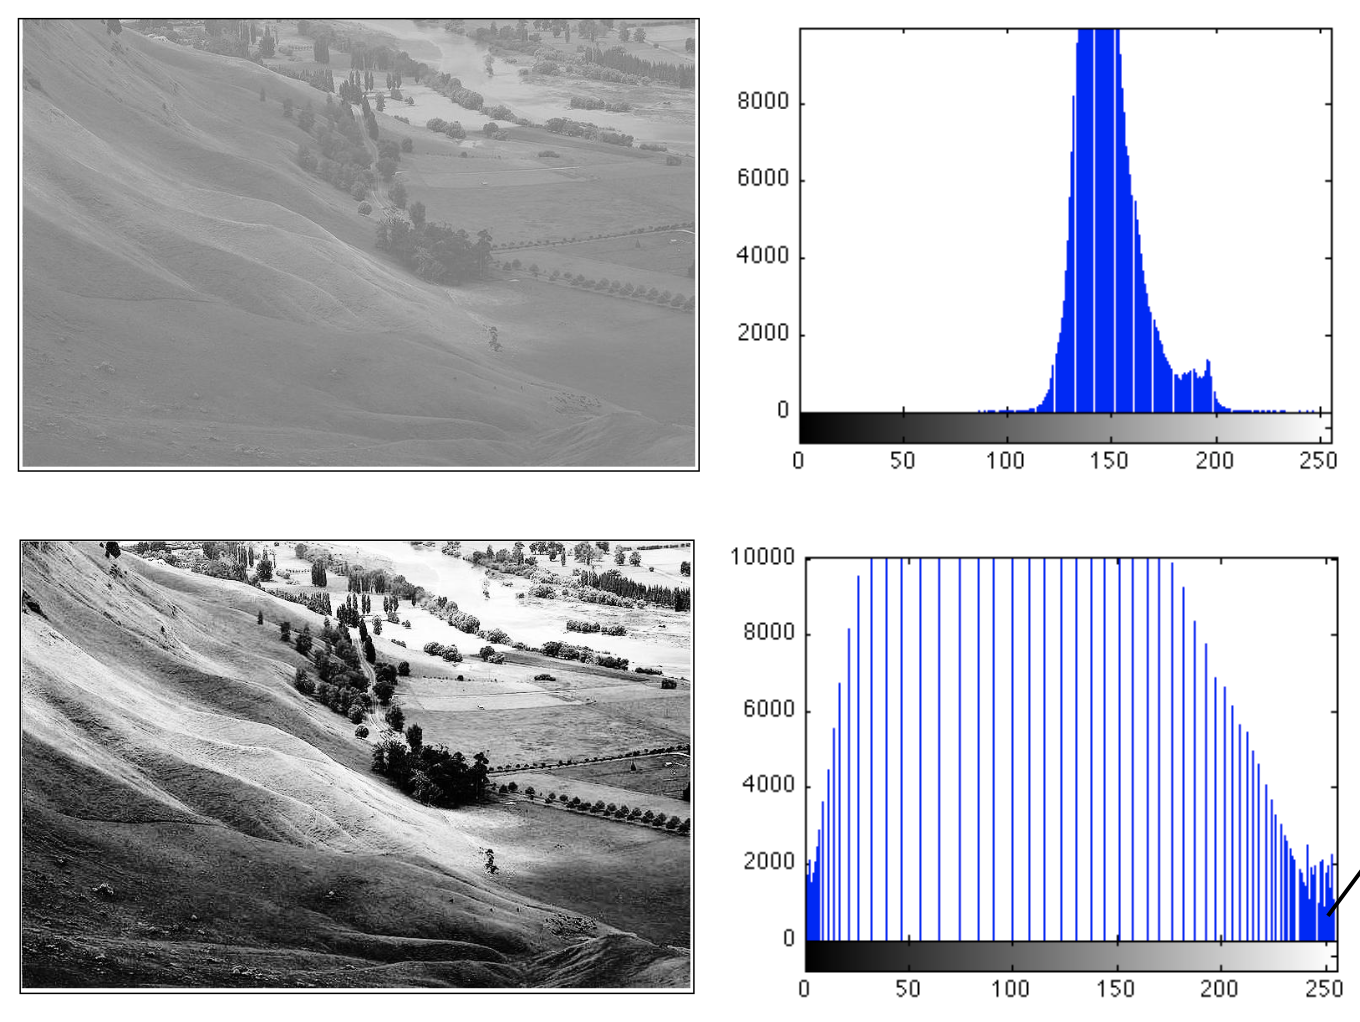
\includegraphics{other/equalization.png}}
  \end{center}
  \caption{Ejemplo de ecualización de una imagen\cite{carrasco1}.} \label{fig:sample_eq}
\end{figure}

En el ejemplo de la Figura \ref{fig:sample_eq} se aprecia que al ecualizar la imagen original se altera el histograma original, aumentando la cantidad de pixeles en los niveles de intensidad bajos y altos.

\subsection{Filtro de la mediana}

El filtro de la mediana corresponde una técnica de filtrado no lineal qué se utiliza para remover ruido de una señal. La idea de este filtro es ir modificando los valores de un pixel en función de sus vecinos. El filtro se aplica a una sub-matriz o máscara de la imagen original, de tamaño impar. El pixel a modificar es el valor central, y su valor se reemplaza por la mediana de todos los valores contenidos en la mascara. La Figura \ref{fig:sample_eq} muestra gráficamente cómo opera el filtro de la mediana, considerando una máscara de 3x3.

\begin{figure}[!tbh]
  \begin{center}
    \resizebox{0.7\columnwidth}{!}{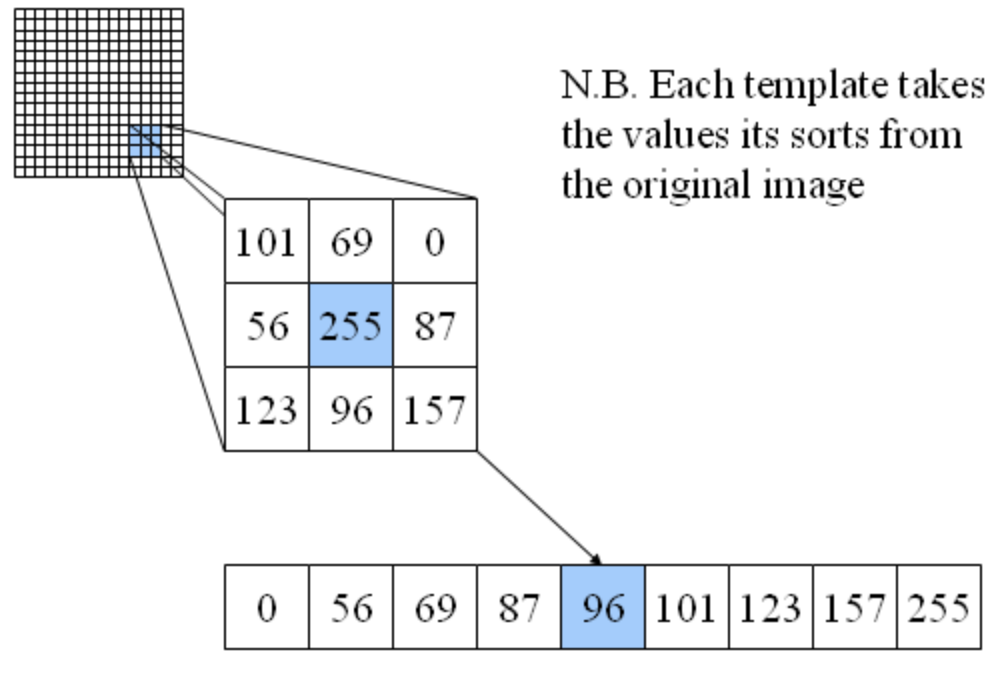
\includegraphics{other/median.png}}
  \end{center}
  \caption{Aplicación filtro de la mediana \cite{median}.} \label{fig:sample_eq}
\end{figure}

\subsection{Binarización de una imagen}

La binarización de una imagen corresponde a convertir los valores de la imagen a solo dos valores posibles: 0 o 1. Esto se realiza considerando una funcion de umbral, la cual determina un intervalo de intensidades que deben ser considerados como True (1), mientras que todo el resto se convierte en False (0).

\[  dst(x,y) = \begin{cases} 
      \text{maxVal} & \text{if} src(x,y) > \text{thresh} \\
      0 & \text{Otro caso} 
   \end{cases}
\]

%%%%%%%%%%%%%%%%%%%%%%%%%%%%%%%%%%%%%%%%%%%%%%%%%%%%%%%%%%%%%%%%%%%%%%%%%%%%%%%%
\section{Imagen original}


Para efectos de este trabajo se manipula la radiografía de una soldadura, con el objetivo de poder identificar las fallas que esta pueda tener. La Figura \ref{fig:original} muestra la imagen original, sin ningún tipo de post-proceso aplicado.

\begin{figure}[!tbh]
  \begin{center}
    \resizebox{\columnwidth}{!}{\includegraphics{outs/input_image.jpg}}
  \end{center}
  \caption{Radiografia de una soldadura.} \label{fig:original}
\end{figure}


%%%%%%%%%%%%%%%%%%%%%%%%%%%%%%%%%%%%%%%%%%%%%%%%%%%%%%%%%%%%%%%%%%%%%%%%%%%%%%%%
\section{Ecualización del Histograma}\label{ecualizacion}

Con el objetivo de mejorar el contraste de la imagen se ecualiza la fotografía. El efecto de realizar esta operación se puede ver claramente al observar el histograma de intensidad de la imagen original versus el de la nueva imagen. En el caso de esta imagen se aumenta la población de pixels en la zonas de mayor intensidad, tal como se puede en la Figura \ref{fig:hist_eq}.

\begin{figure}[!tbh]
  \centering
  \begin{minipage}[b]{0.49\columnwidth}
    \includegraphics[width=\textwidth, trim={0.8cm 0.5cm 0.9cm 1.4cm}, clip]{outs/hist_fallas.png}
    \subcaption{Original}
  \end{minipage}
  % \hfill
  \begin{minipage}[b]{0.49\columnwidth}
    \includegraphics[width=\textwidth, trim={0.8cm 0.5cm 0.9cm 1.4cm}, clip]{outs/hist_fallas_eq.png}
    \subcaption{Ecualizada}
  \end{minipage}
  \caption{Histograma imagen original y ecualizada.} \label{fig:hist_eq}
\end{figure}

\begin{figure}[tbh!]
  \begin{center}
    \resizebox{\columnwidth}{!}{\includegraphics{outs/input_image_eq.jpg}}
  \end{center}
  \caption{Imagen ecualizada.} \label{fig:original_eq}
\end{figure}

%%%%%%%%%%%%%%%%%%%%%%%%%%%%%%%%%%%%%%%%%%%%%%%%%%%%%%%%%%%%%%%%%%%%%%%%%%%%%%%%
\section{Eliminación de ruido}\label{ruido}

Para reducir el ruido presente en la imagen de entrada de se aplica una serie de filtros, cambiando el valor de la mascara a usar. Se explora utilizando valores entre 3 y 80. Algunos resultados se presentan en la Figura \ref{fig:median_grid}.

\begin{figure}[!tbh]
\centering
\includegraphics[width=.3\columnwidth]{outs/median_filter_5.jpg}\quad
\includegraphics[width=.3\columnwidth]{outs/median_filter_11.jpg}\quad
\includegraphics[width=.3\columnwidth]{outs/median_filter_31.jpg}

\medskip

\includegraphics[width=.3\columnwidth]{outs/median_filter_41.jpg}\quad
\includegraphics[width=.3\columnwidth]{outs/median_filter_51.jpg}\quad
\includegraphics[width=.3\columnwidth]{outs/median_filter_61.jpg}

\medskip

\includegraphics[width=.3\columnwidth]{outs/median_filter_67.jpg}\quad
\includegraphics[width=.3\columnwidth]{outs/median_filter_71.jpg}\quad
\includegraphics[width=.3\columnwidth]{outs/median_filter_79.jpg}


\caption{Imagen filtrada mediante filtro de la mediana para distintas máscaras.}
\label{fig:median_grid}
\end{figure}


Como es de esperar, con una mascara mas grande se logra una mayor reducción del ruido, perdiendo los detalles de la imagen. Luego de observar los resultados obtenidos se opta por generar una imagen con un filtro de la mediana con una máscara de 77x77.

%La imagen completa filtrada se presenta en la Figura \ref{fig:median}.

%\begin{figure}[!tbh]
%  \begin{center}
%    \resizebox{\columnwidth}{!}{\includegraphics{outs/median_filter_77_completo.jpg}}
%  \end{center}
%  \caption{Imagen filtrada mediante filtro de la mediana 71x71.} \label{fig:median}
%\end{figure}


%%%%%%%%%%%%%%%%%%%%%%%%%%%%%%%%%%%%%%%%%%%%%%%%%%%%%%%%%%%%%%%%%%%%%%%%%%%%%%%%%
\section{Combinación imagen filtrada y ecualizada}\label{p4}

Utilizando las imagenes generadas en \ref{ecualizacion} y \ref{ruido} se crea una nueva imagen considerando la resta de ambas imágenes (imagen\textsubscript{mediana} - imagen\textsubscript{ecualizada}). En la Figura \ref{fig:pregunta4} se presenta el resultado de la operación aritmética entre ambas imágenes.

A través de este proceso se logra identificar la zonas en las cuales la soldadura presenta errores. El resultado se logra ver de mejor forma al interpretar la imagen utilizando una escala de colores, como se muestra en la Figura \ref{fig:pregunta4color}.


\begin{figure}[!tbh]
\centering
\begin{subfigure}[b]{\columnwidth}
 	\includegraphics[width=1\linewidth]{outs/img_p4}
 	\subcaption{Escala de grises}
  	\label{fig:pregunta4}
\end{subfigure}
\begin{subfigure}[b]{\columnwidth}
 	\includegraphics[width=1\linewidth]{outs/img_p4_color.jpg}
  	\subcaption{Pseudocolor}
  	\label{fig:pregunta4color}
\end{subfigure}
\caption{Imagen compuesta utilizando las imágenes de \ref{ecualizacion} y \ref{ruido}.}
\label{fig:p4_both}
\end{figure}


%%%%%%%%%%%%%%%%%%%%%%%%%%%%%%%%%%%%%%%%%%%%%%%%%%%%%%%%%%%%%%%%%%%%%%%%%%%%%%%%%
\section{Binarización de la imagen}\label{bin}


De la imagen de la Figura \ref{fig:pregunta4} se tiene que la imagen presenta zonas oscuras y zonas claras. Se prueba valores en el intervalo [1, 55] y algunos resultados se muestran en la Figura \ref{fig:threshold_grid}.


\begin{figure}[!tbh]
\centering
\includegraphics[width=.3\columnwidth]{outs/img_p5_threshold_2.jpg}\quad
\includegraphics[width=.3\columnwidth]{outs/img_p5_threshold_10.jpg}\quad
\includegraphics[width=.3\columnwidth]{outs/img_p5_threshold_20.jpg}

\medskip

\includegraphics[width=.3\columnwidth]{outs/img_p5_threshold_30.jpg}\quad
\includegraphics[width=.3\columnwidth]{outs/img_p5_threshold_40.jpg}\quad
\includegraphics[width=.3\columnwidth]{outs/img_p5_threshold_50.jpg}

 \caption{Imagen filtrada mediante filtro de la mediana para distintas máscaras.}
 \label{fig:threshold_grid}
\end{figure}

Elegir un valor umbral muy alto descarta posibles zonas donde la soldadura presenta errores, mientras que los valores bajos identifican la zona del borde superior fallas en soldadura. De la inspección de todos los resultados se decide usar un umbral de 10 en los pasos posteriores.


%%%%%%%%%%%%%%%%%%%%%%%%%%%%%%%%%%%%%%%%%%%%%%%%%%%%%%%%%%%%%%%%%%%%%%%%%%%%%%%%%
\section{Resultados finales}

Finalmente se multiplica la imagen ecualizada de \ref{ecualizacion} con la imagen binaria resultante de \ref{bin}. La imagen binaria posee valores de True y False, donde los valores True indican las zonas donde la soldadura presenta fallas. Al multiplicar esto con la imagen de \ref{ecualizacion} básicamente se "apagan" todos los puntos que no son de interés en la imagen. Esto es el equivalente al haber cortado una plantilla marcando las areas deseadas, para luego poner esta plantilla sobre la imagen original.

\begin{figure}[!tbh]
\centering
\begin{subfigure}[b]{\columnwidth}
   \includegraphics[width=1\linewidth]{outs/input_image.jpg}
   \caption{Imagen original}
   \label{fig:Ng1}
\end{subfigure}

\begin{subfigure}[b]{\columnwidth}
   \includegraphics[width=1\linewidth]{outs/img_final.jpg}
   \caption{Imagen final}
   \label{fig:Ng2}
\end{subfigure}
 \caption{Comparación imagen de entrada y resultado final.} \label{fig:img_final}
\end{figure}


%%%%%%%%%%%%%%%%%%%%%%%%%%%%%%%%%%%%%%%%%%%%%%%%%%%%%%%%%%%%%%%%%%%%%%%%%%%%%%%%
\section{Manual uso}

En conjunto a este documento se entrega el código fuente asociado al
desarrollo de este trabajo.

Para recrear los resultados obtenidos en este documento basta con
ejecutar el script \texttt{Tarea\_2.py} agregando como opción la
pregunta asociada.

\begin{verbatim}
# Ejecuta pregunta 1
Tarea_2.py P1

# Ejecuta todo
Tarea_2.py ALL
\end{verbatim}






\nocite{*}
\bibliographystyle{IEEEtran}
\bibliography{bibliography}


\end{document}



%\begin{lstlisting}[language=bash]
%  $ wget http://tex.stackexchange.com
%\end{lstlisting}

%\begin{table} \caption{A Simple Example Table} \label{table_example}
%  \begin{center}
%    \begin{tabular}{c c}
%      \hline
%      \bfseries First & \bfseries Next\\ \hline\hline
%      1.0 & 2.0 \\
%      \hline
%    \end{tabular}
%  \end{center}
%\end{table}

%\begin{figure}[tbh!]
%\begin{center}
%\psfragscanon
%\psfrag{Impulso}[Bc][Br][1.6]{Impulso.}
%\psfrag{Resp impulse}[Bc][Br][1.6]{Respuesta a impulso de $H(z)$.}
%\psfrag{Amplitud}[Bc][Br][1.6]{Amplitud}
%\psfrag{N}[Bc][Br][1.6]{Número de muestra}
%\resizebox{0.5\columnwidth}{!}{\includegraphics{./mfiles/part1/resp_impulse_IIR_parte02.eps}}
%\end{center}
%\caption{Respuesta a impulso del filtro IIR.}
%\label{fig:resp imp IIR}
%\end{figure}

%\begin{lstlisting}[float=tbh!, caption={Magnitud de la respuesta en frecuencia del filtro IIR},label={cod:mag resp frec %IIR}]
%mag=20*log10(abs(H));
%\end{lstlisting}